\chapter{Karplus}
\label{Karplus}
\section{Notizen}



Karplus strong und PM,\\
schwingungssysteme,\\
simulation..

Ableton Live: donner,\\
rechtfertigung: Computerspiele, etc.\\
(Wellen-)Experiment.\\
Geschichte: Bernoulli und D'Alembert\\
Wellengleichung
Karplus Strong (bauen, geschichte erzählen)
(Pause)
Waveguide, Scattering Junctions erwähnen undje nach interesse behandeln. Kelly und Lochbaum modell.
Kaffeehäferl synthetisieren. (Praat, reson)



\section{Vorbereitung}


Konzeptuelle Gedanken(imaginary number, complex numbers): \\
https:\/\/www.youtube.com\/watch?v=-IJuqR6nz\_Q \\
https:\/\/www.youtube.com\/watch?v=EIstpPXKWng
wellengleichung:\\
https:\/\/www.youtube.com\/watch?v=Li6OEMCtQ9k




\section{Uebersicht}


\begin{enumerate}
	\item motivation: gewitter im ableton live
	\item PM: erklärung
	\item Karplus strong 
	\item Schulübung: sounddesign challenge in pd.

\end{enumerate}

\section{Theorie, Schwingungsfähige systeme}


Wellengleichung, unendliche eindimensionale saite:
\begin{equation}
	c^2 \cdot \frac{\delta^2 f}{\delta x^2} = \frac{\delta ^2 f}{\delta t ^2}
\end{equation}

Visualisierung:

\begin{figure}[H]
  \begin{center}
    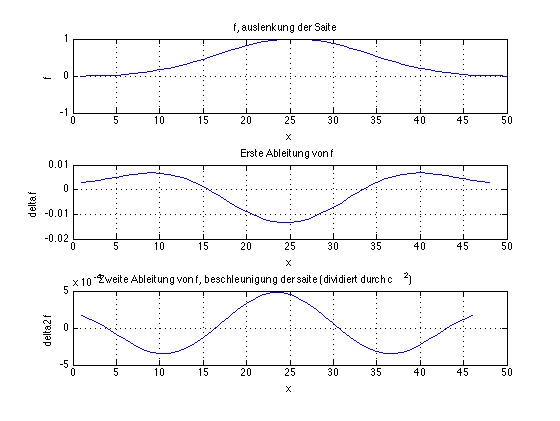
\includegraphics[width = 14cm]{img/wellengleichung.png}
    \caption{Visualisierung der Wellengleichung}
    \label{fig:wellengleichung}
  \end{center}
\end{figure}




Zwei lösungs ansätze: 
\begin{itemize}
	\item Bernoulli = ca. fourier, spectral, summe von sinus schwingungen.
	\item D'Alembert = ca. Physical modeling, zwei funktionen die entlang der saite reisen (in entgegengesetzte richtung).
\end{itemize}


\begin{equation}
y(x, t) = y ^+ \Bigg(t - \frac{x}{c}\Bigg) + y^- \Bigg(t + \frac{x}{c} \Bigg)
\end{equation}

D'Alembert sagt also, es gäbe zwei wellen, die in zwei richtungen entlang der saite reisen, die Lässt sich einfach simulieren, mittels zwei in einander geschalteten delays.

\section{Parktical Karplus-Strong}
\begin{figure}[h]
	\begin{center}
		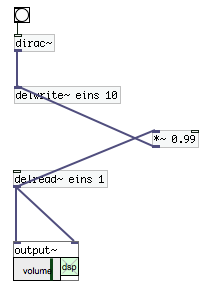
\includegraphics[scale = 1.]{img/karplusSimple.png}
		\caption{Basic setup}
		\label{fig:karplusBasic}
	\end{center}
\end{figure}

  \begin{figure}[htb]
  \centering  
  \caption{grundsätzlches Waveguide/Karplus Strong Modell.}
  \label{fig:string}

  % \resizebox{10cm}{!}{%
  \begin{tikzpicture}[auto, thick, node distance=2.3cm, >=triangle 45]

  \draw node at (5,0) [block] (del1) {\Large$\ \ \ \ \ \ \ \ z^{-m}\ \ \ \ \ \ \ \ $};
  \draw node at (5,-3) [block] (del2) {\Large$\ \ \ \ \ \ \ \ z^{-m}\ \ \ \ \ \ \ \ $};
  \draw node at (0, -1.5) [mult] (m1) {\Large$-1$};
  \draw node at (10, -1.5) [mult] (m2) {\Large$-1$};

  \draw[->] (del1) -| node {}(m2);
  \draw[->] (m2) |- node {}(del2);
  \draw[->] (del2) -| node {}(m1);
  \draw[->] (m1) |- node {}(del1);
	
  \end{tikzpicture}
  % }
\end{figure}

\begin{figure}[htb]
  \centering  
  \caption{einzelne Saite, $G(z)$ ein lowpass, \glqq{}Loss Filter\grqq{}}
  \label{fig:string}

  \begin{tikzpicture}[auto, thick, node distance=2.3cm, >=triangle 45]

  \draw node at (0,0) [input] (excitation) {};
  \draw node [sum, right of=excitation, node distance = 2.cm] (sum1) {\Large$+$};
  \draw node [block, right of=sum1, node distance = 2cm] (delay) {\Large$z^{-m}$};
  \draw node [block, below of=delay, node distance = 2cm] (loss) {\Large$G(z)$};
  \draw node at (6.,-0.001) {\textbullet};

  \draw node [output, right of=delay,node distance = 3cm] (out) {};
  \draw[->] (excitation) -- node {\Large$x[n]$}(sum1);
  \draw[->] (sum1) -- node {}(delay);
  \draw[->] (loss.west) -| node {}(sum1.south);

  \draw[->] (6., -0.001) |- node {}(loss.east);


  \draw[->] (delay) -- node {\Large$y[n]$}(out);
    
  \end{tikzpicture}
\end{figure}


\section{Schulübung, Sounddesign challenge}
zB:
\begin{itemize}
	\item Vokal
	\item E-gitarre
	\item beliebiges Physikalisches object

\end{itemize}
	
\section{Hausuebung}
Andy Farnell, \href{http://aspress.co.uk/ds/pdf/pd_intro.pdf}{pd intro} chater 7, lesen

    